\chapter{\label{chap:related-work}Trabalhos Relacionados}
As tarefas de criar uma inteligência artificial para personagens em jogos
digitais e de criar agentes inteligentes capazes de aprender a jogar jogos
digitais já foram exploradas em outros trabalhos. Neste capítulo, selecionamos
alguns trabalhos que se propuseram a resolver estas tarefas, indicando sua
relevância e similaridade com o projeto presente neste trabalho. 


%----------
\section{Playing Atari with Deep Reinforcement Learning}
O artigo apresenta um modelo de \textit{deep learning} capaz de aprender
políticas de controle para sete jogos do \textit{console} Atari 2600, criando
uma inteligência artificial capaz de jogar eficientemente todos os jogos,
inclusive superando jogadores humanos em alguns deles
\cite{DBLP:journals/corr/MnihKSGAWR13}. O modelo utiliza aprendizado por reforço
e uma rede neural convolucional treinada com uma variante de \textit{Q-learning}
para criar o agente. Para criar estas políticas de controle, os autores
utilizaram uma plataforma de testes de inteligência artificial chamada
\textit{Arcade Learning
Environment}\footnote{http://www.arcadelearningenvironment.org/}, ou
\textit{ALE}.

O treinamento se deu através da utilização dos valores dos \textit{pixels}
apresentados na tela. Como as informações do estado do jogo eram altamente
dimensionais, a utilização de \textit{deep learning} e redes neurais
convolucionais provou ser uma excelente -- e necessária -- escolha para realizar
o treinamento do agente. Contudo, o treinamento do agente utilizando esta
técnica é extremamente demorado.

Como a dimensionalidade do estado do jogo fornecido pela ferramenta
\textit{SpelunkBots} não é tão grande quanto a do trabalho em questão, optamos
por não fazer uso de \textit{deep learning}, mesmo que a técnica também seja
muito promissora.


%----------
\section{A Neuroevolution Approach to General Atari Game Playing}
Este artigo apresenta uma série de abordagens neuroevolutivas
(\textit{Conventional Neuroevolution}, \textit{Covariance Matrix Adaptation
Evolution Strategy}, \textit{Neuroevolution of Augmenting Topologies} e
\textit{Hypercube-based Neuroevolution of Augmenting Topologies}\footnote{O
\textit{HyperNEAT} é uma extensão do algoritmo \textit{NEAT} utilizado para
evoluir redes neurais de grande escala utilizando regularidades geométricas do
domínio do problema.}) para realizar a criação de agentes inteligentes capazes
de aprender a jogar jogos do \textit{console} \textit{Atari 2600} com pouco
conhecimento específico sobre os domínios dos jogos \cite{NeuroEvolutionAtari}.
Este trabalho também utiliza a ferramenta \textit{ALE}.

Os autores realizaram a representação de estados dos jogos de três maneiras
distintas: objetos da tela de jogo, os \textit{pixels} da tela e ruído.  A
representação por ruído foi utilizada para servir como base de comparação e
investigar quanto do aprendizado é baseado na memorização e em conceitos gerais.

As políticas de controle evoluídas através de algoritmos neuroevolutivos atingem
resultados excelentes e, em alguns jogos, superam o desempenho de jogadores
humanos, sugerindo que a neuroevolução é uma abordagem promissora para criação
de agentes inteligentes e \textit{general video game playing} (criar um agente
que seja capaz de jogar diversos jogos digitais sem mudanças de parâmetros). Os
algoritmos com os melhores resultados, em todas as categorias de representação
de estados, foram o \textit{NEAT} e \textit{HyperNEAT}.


%----------
\section{Creating Artificial Intelligence Agents for \textit{Spelunky} using an
Artificial Neural Network and a Genetic Algorithm}
Este trabalho apresenta o desenvolvimento de uma inteligência artificial para o
jogo \textit{Spelunky}, através da utilização de redes neurais e algoritmos
genéticos, cujo objetivo é navegar da entrada até a saída de cenários de testes
estipulados \cite{spelunky_ann_genetic}. Para tal, o autor utiliza o
\textit{framework} de Inteligência Artificial \textit{SpelunkBots}.

A rede neural utilizada é uma simples rede sem realimentação
(\textit{feed-forward}) de topologia fixa com as seguintes características:

\begin{itemize}
	\item \textbf{Entrada:} A rede possui 4 nodos de entrada: distância do
		jogador até o objetivo, altura do objetivo em relação ao jogador,
		direção do objetivo em relação ao jogador e a existência de obstáculos
		no caminho do jogador.
	
	\item \textbf{Camadas Escondidas:} Duas camadas escondidas, com 4 nodos
		cada.

	\item \textbf{Saídas:} 4 nodos de saída, cada um mapeado para uma
		característica de um nodo de entrada. Por exemplo, um nodo de saída para
		distância do jogador até o objetivo.

	\item \textbf{Conexões:} Os nodos de uma camada são conectados
		todos-para-todos com os nodos da camada seguinte.

	\item \textbf{Pesos:} Os pesos das conexões apresentavam valores entre -1 e
		1.

	\item \textbf{Função de Ativação:} A função de ativação utilizada é do tipo
		sigmóide, mais especificamente uma modificação da função \textit{tanh}:
		$((e^{x} - e^{-x})/2) / ((e^{x} + e^{-x})/2)$. Esta função normaliza os
		valores, restringindo-os entre -1 e 1.
\end{itemize}

O algoritmo de seleção de indivíduos do algoritmo genético escolhido pelo autor
é o \textit{tournament selection}. A função de aptidão escolhida para mensurar a
qualidade dos agentes se baseia na distância do agente até a saída e o tempo
necessário para completar o nível. Com o objetivo de testar a eficácia das
técnicas escolhidas, o autor desenvolveu 10 cenários de teste, executou os
agentes em cada um deles e coletou resultados destas execuções para análise. É
importante ressaltar que os cenários escolhidos pelo autor eram extremamente
simples e não correspondem com um mapa gerado proceduralmente pelo jogo.

Apesar de ser capaz de gerar agentes aptos a chegar ao fim de todos os níveis,
muitas vezes os agentes criados nos mapas mais avançados não eram capazes de
vencer os mapas mais simples. O autor relata, em suas considerações finais que a
habilidade do algoritmo genético escolhido de selecionar agentes adequados para
mutação e reprodução era limitada. O autor crê que não era possível identificar
se esta característica era um ponto negativo ou não porque deve existir um
\textit{trade-off} entre modificar agentes, pois modificando muito correria o
risco de perder características boas e modificando pouco poderia ficar com baixa
diversidade genética. 


%----------
\section{MCTS \textit{Spelunky}: A comparison on the use of Forward-Facing
Artificial Intelligence Algorithms with Artificial Intelligence Bots in
\textit{Spelunky}}
O objetivo deste trabalho era investigar a viabilidade de se criar um agente
inteligente para o jogo \textit{Spelunky} utilizando o algoritmo de busca
\textit{Monte-Carlo Tree Search}, que já foi utilizado em jogos como \textit{Go}
e \textit{StarCraft} \cite{spelunky_mcts}. Este trabalho também utiliza a
ferramenta \textit{SpelunkBots}.

O autor desenvolveu 3 cenários de teste para identificar limitações da
aplicabilidade da técnica. Após, utilizou os \textit{bots} padrões inclusos na
ferramenta \textit{SpelunkBots} a fim de comparar os resultados obtidos. 

Um ponto importante a ser ressaltado deste trabalho é que os cenários de teste
desenvolvidos eram extremamente simplistas e que a comparação entre o agente do
autor com os \textit{bots} padrões da ferramenta era injusta, pois o propósito
de muitos destes \textit{bots} é apenas ilustrar o uso da \textit{API} para
novos desenvolvedores. Estes \textit{bots}, inclusive, possuem comportamentos
fixos e em alguns testes nem chegaram a executar de fato. Mesmo assim, o agente
desenvolvido pelo autor também foi incapaz de superar 2 dos 3 cenários de teste,
pois o programa tornava-se irresponsivo após alguns segundos de execução, o que
é atribuido ao autor como uma falha de implementação, e não uma escolha ruim de
algoritmo.


%----------
\section{MarI/O}
Em junho de 2015, o canal do \textit{YouTube}
SethBling\footnote{https://www.youtube.com/user/sethbling/about} divulgou
o vídeo \textit{MarI/O - Machine Learning for Video
Games}\footnote{https://www.youtube.com/watch?v=qv6UVOQ0F44}, onde utilizava a
técnica \textit{NEAT} para criar a inteligência artificial de um agente para o
jogo \textit{Super Mario World}.

\begin{figure}[htb!]
\centering
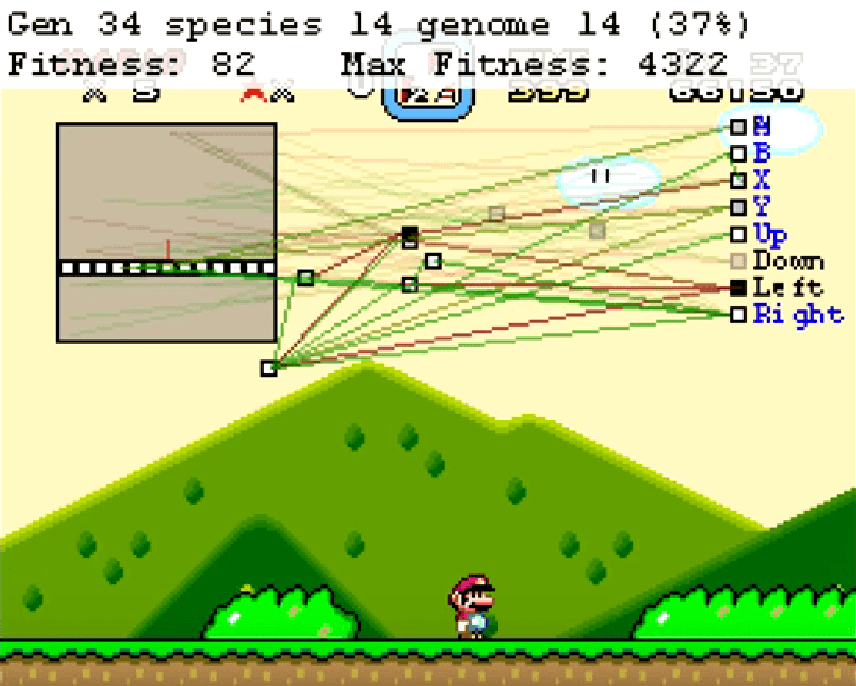
\includegraphics[width=.65\textwidth]{fig/mar-io-example.pdf}
\caption{\label{fig:mar-io-example}Exemplo da visão do jogo \textit{Super
Mario World} através do projeto \textit{MarI/O}, mostrando elementos de
controle usados pelo NEAT, como a rede neural, as possíveis ações, as
gerações, as espécies, os genomas, entre outros.}
\end{figure}

Depois do sucesso da aplicação da técnica no jogo \textit{Super Mario World}, o
autor decidiu aplicar a técnica em outros dois jogos da franquia \textit{Mario}:
\textit{Super Mario Bros.}\footnote{https://www.youtube.com/watch?v=iakFfOmanJU}
e \textit{Super Mario
Kart}\footnote{https://www.youtube.com/watch?v=S9Y\_I9vY8Qw}. Também foi
possível, nestes outros jogos, criar agentes capazes de jogar de maneira
autônoma.

Nos jogos escolhidos por SethBling, os níveis são sempre os mesmos, o que torna
mais fácil medir o desempenho dos agentes, pois a disposição do nível é sempre
igual e o objetivo final sempre se encontra no mesmo lugar. Este não é o caso em
\textit{Spelunky}, onde os níveis são gerados proceduralmente. Além disso, os
níveis de \textit{Super Mario World} e \textit{Super Mario Bros.} são
essencialmente horizontais e movimentar o personagem para a direita quase sempre
garante alguma forma de progresso. Em \textit{Spelunky} não é possível saber de
antemão onde se encontra a saída do nível e o movimento horizontal não garante o
progresso, visto que os níveis não são essencialmente horizontais. 
